%%%%%%%%%%%%%%%%%%%%%%%%%%%%%%%%%%%%%%%%%%%%%%%
%%%     Declarations (skip to Begin Document, line 88, for parts you fill in)
%%%%%%%%%%%%%%%%%%%%%%%%%%%%%%%%%%%%%%%%%%%%%%%

\documentclass[10pt]{article}

\usepackage{geometry}  % Lots of layout options.  See http://en.wikibooks.org/wiki/LaTeX/Page_Layout
\geometry{letterpaper}  % ... or a4paper or a5paper or ... 
\usepackage{fullpage}  % somewhat standardized smaller margins (around an inch)
\usepackage{setspace}  % control line spacing in latex documents
\usepackage[parfill]{parskip}  % Activate to begin paragraphs with an empty line rather than an indent

\usepackage{amsmath,amssymb}  % latex math
\usepackage{empheq} % http://www.ctan.org/pkg/empheq
\usepackage{bm,upgreek}  % allows you to write bold greek letters (upper & lower case)

% for typsetting algorithm pseudocode see http://en.wikibooks.org/wiki/LaTeX/Algorithms_and_Pseudocode
\usepackage{algorithmic,algorithm}  

\usepackage{graphicx}  % inclusion of graphics; see: http://en.wikibooks.org/wiki/LaTeX/Importing_Graphics
% allow easy inclusion of .tif, .png graphics
\DeclareGraphicsRule{.tif}{png}{.png}{`convert #1 `dirname #1`/`basename #1 .tif`.png}

\usepackage{subfigure}  % allows subfigures in figure

\usepackage{xspace}
\newcommand{\latex}{\LaTeX\xspace}

\usepackage{color}  % http://en.wikibooks.org/wiki/LaTeX/Colors

\long\def\ans#1{{\color{blue}{\em #1}}}
\long\def\ansnem#1{{\color{blue}#1}}
\long\def\boldred#1{{\color{red}{\bf #1}}}
\long\def\boldred#1{\textcolor{red}{\bf #1}}
\long\def\boldblue#1{\textcolor{blue}{\bf #1}}

% Useful package for syntax highlighting of specific code (such as python) -- see below
\usepackage{listings}  % http://en.wikibooks.org/wiki/LaTeX/Packages/Listings
\usepackage{textcomp}

%%% The following lines set up using the listings package
\renewcommand{\lstlistlistingname}{Code Listings}
\renewcommand{\lstlistingname}{Code Listing}

%%% Specific for python listings
\definecolor{gray}{gray}{0.5}
\definecolor{green}{rgb}{0,0.5,0}

\lstnewenvironment{python}[1][]{
\lstset{
language=python,
basicstyle=\footnotesize,  % could also use this -- a little larger \ttfamily\small\setstretch{1},
stringstyle=\color{red},
showstringspaces=false,
alsoletter={1234567890},
otherkeywords={\ , \}, \{},
keywordstyle=\color{blue},
emph={access,and,break,class,continue,def,del,elif ,else,%
except,exec,finally,for,from,global,if,import,in,i s,%
lambda,not,or,pass,print,raise,return,try,while},
emphstyle=\color{black}\bfseries,
emph={[2]True, False, None, self},
emphstyle=[2]\color{green},
emph={[3]from, import, as},
emphstyle=[3]\color{blue},
upquote=true,
morecomment=[s]{"""}{"""},
commentstyle=\color{gray}\slshape,
emph={[4]1, 2, 3, 4, 5, 6, 7, 8, 9, 0},
emphstyle=[4]\color{blue},
literate=*{:}{{\textcolor{blue}:}}{1}%
{=}{{\textcolor{blue}=}}{1}%
{-}{{\textcolor{blue}-}}{1}%
{+}{{\textcolor{blue}+}}{1}%
{*}{{\textcolor{blue}*}}{1}%
{!}{{\textcolor{blue}!}}{1}%
{(}{{\textcolor{blue}(}}{1}%
{)}{{\textcolor{blue})}}{1}%
{[}{{\textcolor{blue}[}}{1}%
{]}{{\textcolor{blue}]}}{1}%
{<}{{\textcolor{blue}<}}{1}%
{>}{{\textcolor{blue}>}}{1},%
%framexleftmargin=1mm, framextopmargin=1mm, frame=shadowbox, rulesepcolor=\color{blue},#1
framexleftmargin=1mm, framextopmargin=1mm, frame=single,#1
}}{}
%%% End python code listing definitions

\DeclareMathOperator{\diag}{diag}
\DeclareMathOperator{\cov}{cov}

%%%%%%%%%%%%%%%%%%%%%%%%%%%%%%%%%%%%%%%%%%%%%%%
%%%     Begin Document
%%%%%%%%%%%%%%%%%%%%%%%%%%%%%%%%%%%%%%%%%%%%%%%

\begin{document}

\begin{center}
    {\Large {\bf ISTA 421/521 -- Homework 3}} \\
    \boldred{Due: Friday, October 11, 10pm} \\
    20 pts total for Undergrads, 25 pts total for Grads
\end{center}

\begin{flushright}
STUDENT NAME %% Fill in your name here

Undergraduate / Graduate %% select which you are!
\end{flushright}

\vspace{1cm}
{\Large {\bf Instructions}}

In this assignment you are required to modify/write 2 scripts in python.  They will be submitted as 2 separate files, although you are free to copy chunks of code from any other script, especially the example scripts being provided in this homework.  Details of what you are to do are specified in problems 2 and 7, below.

Included in the homework 3 release are following sample scripts:
\begin{itemize}
\item {\tt approx\_expected\_value.py} - This script demonstrates how to approximate an expected value through sampling.  You will modify this code and submit your solution for problem 2.
\item {\tt gauss\_surf.py} - This is provided for fun -- it is not required for any problem here.  It generates a 2d multivariate Gaussian and plots it as both a contour and surface plots.  In later work in this class, we will use contour plots.
\item {\tt predictive\_variance\_example.py} - This script demonstrates (a) generating and plotting error bars (predictive variance) and (b) sampling of model parameters from the $\cov\{\widehat{\mathbf{w}}\}$ estimated from data.  You will run this script in problem 6, and then use it as the basis for a script in problem 7.
\item {\tt w\_variation\_demo.py} - This script is also provided for fun and is not required for the assignment.  However, it provides more python code as an example.  This implements the simulated experiment demonstrating the theoretical and empirical bias in the estimate of variance, $\widehat{\sigma^2}$, of the model variance, $\sigma^2$, as a function of the sample size used for estimation.
\end{itemize}

All problems require that you provide some ``written'' answer (in some cases also figures), so you will also submit a .pdf of your written answers.  (You can use \latex or any other system (including handwritten; plots, of course, must be program-generated) as long as the final version is in PDF.)

\boldred{The final submission will include (minimally) the two scripts and a PDF version of your written part of the assignment.  You are required to create either a .zip or tarball (.tar.gz / .tgz) archive of all of the files for your submission and submit your archive to the d2l dropbox by the date/time deadline above.}

NOTE: Problems 4 and 8 are required for Graduate students only; Undergraduates may complete them for extra credit equal to the point value.

(FCMA refers to the course text: Rogers and Girolami (2012), {\em A First Course in Machine Learning}.  For general notes on using \latex to typeset math, see: {\tt http://en.wikibooks.org/wiki/LaTeX/Mathematics})
\vspace{.5cm}

%%%%%%%%%%%%%%%%
%%%     Problems
%%%%%%%%%%%%%%%%

\newpage
\begin{itemize}

%%%     Problem 1
\item[1.] [2 points]
Adapted from {\bf Exercise 2.3} of FCMA p.90:

Let $Y$ be a random variable that can take any positive integer value.  The likelihood of these outcomes is given by the Poisson pdf:
\begin{eqnarray}
p(y) = {\lambda^y\over y!} e^{-\lambda}
\end{eqnarray}
By using the fact that for a discrete random variable the pdf gives the probabilities of the individual events occurring and the probabilities are additive...
\begin{enumerate}
\item[(a)] Compute the probability that $Y \leq 5$ for $\lambda = 7$, i.e., $P(Y \leq 5)$.  Write a (very!) short python script to compute this value, and include a listing of the code in your solution.
\item[(b)] Using the result of (a) and the fact that one outcome has to happen, compute the probability that $Y > 5$.
\end{enumerate}

{\bf Solution.} 
\\a)
\begin{verbatim}
numpy as np
import matplotlib.pyplot as plt

y = 5 ## value for parameter y as defined in assignment
lamb = 7 ## value for parameter lambda as defined in assignment
answer = 0  ## declaring what will become the answer to problem
for x in range(0,y+1):
    e = np.exp(-lamb)
    fact = 1
    for i in range(1,x+1):
        fact = fact * i

    num = lamb ** x
    den = fact

    frac = num/den
    inst = frac * e ##instance

    answer = answer + inst

print('The probability that y is less than or euqal to ' + str(y) + ' is ' +  str(answer))
print('The probability that y is greater than ' + str(y) + ' is ' + str(1-answer))

\end{verbatim}


 $P(Y \le 5) = 0.300009166667$
 
 b)
 \\$P(Y  > 5) = [1-P(Y \le 5)]= 0.699990833333$


%%%     Problem 2
\item[2.] [3 points]
Adapted from {\bf Exercise 2.4} of FCMA p.90:

Let $Y$ be a random variable with uniform density, $p(y) = \mathcal{U}(a,b)$.  Derive $\mathbf{E}_{p(y)} \{ \sin(y) \}$.  Note that $\int \sin(y)~dy = - \cos(y)$.  Compute $\mathbf{E}_{p(y)} \left\{ \sin(y) \right\}$ for $a=0$, $b=1$ (show the steps).  

The script {\tt approx\_expected\_value.py} demonstrates how you use random samples to approximate an expectation, as described in Section 2.5.1 of the book.  In this case, the script estimates the expectation of the function $x^2$ when $X \sim \mathcal{U}(0,1)$ (that is, $y$ is uniformly distributed between $0$ and $1$).  This script shows a plot of how the estimation improves as larger samples are considered, up to 100 samples.

Modify the script {\tt approx\_expected\_value.py} to compute a sample-based approximation to this expectation of the function $\sin(y)$ when $Y \sim \mathcal{U}(0,1)$ and observe how the approximation improves with the number of samples drawn.  Include a plot showing the evolution of the approximation, relative to the true value, over 3,000 samples.

{\bf Solution.}


\[E_{P(y)} = \int_0^1 \sin(y) P(y) \, dy = \left. {{-\cos(y)} \over {b - a}} \right |_0^1 =  {{-\cos(1)+\cos(0)} \over {1 - 0} } =  0.45969769413186023\]
%\begin{figure}[htb]
%\begin{center}
%\includegraphics[width=8cm]{figs/###}
%\caption{Your caption here}
%\end{center}
%\end{figure}


%%%     Problem 3
\item[3.] [3 points]
Adapted from {\bf Exercise 2.5} of FCMA p.91:

Assume that $p(\mathbf{w})$ is the Gaussian pdf for a $D$-dimensional vector $\mathbf{w}$ given in
\begin{eqnarray*}
p(\mathbf{w}) = \frac{1}{(2 \pi)^{D/2} | \mathbf{\Sigma} |^{1/2}} \exp \left\{ -\frac{1}{2} (\mathbf{w} - \mathbf{\mu})^\top \mathbf{\Sigma}^{-1} (\mathbf{w} - \mathbf{\mu}) \right\} .
\end{eqnarray*}
By expanding the vector notation and re-arranging, show that using $\mathbf{\Sigma} = \sigma^2 \mathbf{I}$ as the covariance matrix, assumes independence of the $D$ elements of $\mathbf{w}$.  You will need to be aware that the determinant of a matrix that only has entries on the diagonal ($|\sigma^2 \mathbf{I}|$) is the product of the diagonal values and that the inverse of the same matrix is constructed by simply inverting each element on the diagonal.  (Hint, a product of exponentials can be expressed as an exponential of a sum.  Also, just a reminder that $\exp\{x\}$ is $e^x$.)

{\bf Solution.} 

\begin{eqnarray*}
p(\mathbf{w}) = \frac{1}{(2 \pi)^{D/2} {{\begin{bmatrix} \sigma^2 & 0\\ 0 & \sigma^2 \end{bmatrix}} } ^{1/2}} \exp \left\{ -\frac{1}{2} (\mathbf{w} - \mathbf{\mu})^\top \mathbf{{\begin{bmatrix} {1 \over \sigma^2} & 0\\ 0 & { 1 \over \sigma^2} \end{bmatrix}} }(\mathbf{w} - \mathbf{\mu}) \right\} .
\end{eqnarray*}


%%%     Problem 4
\item[4.] [2 points; \boldred{Required only for Graduates}]
Adapted from {\bf Exercise 2.6} of FCMA p.91:

Using the same setup as in Problem 4, see what happens if we use a diagonal covariance matrix with different elements on the diagonal, i.e.,
\begin{eqnarray*}
\mathbf{\Sigma} = 
\begin{bmatrix}
\sigma_1^2 & 0 & \cdots & 0 \\
0 & \sigma_2^2 & \cdots & 0 \\
\vdots & \vdots & \ddots & \vdots \\
0 & 0 & \cdots & \sigma_D^2
\end{bmatrix}
\end{eqnarray*}

{\bf Solution.} $<$Solution goes here$>$


%%%     Problem 5
\item[5.] [4 points]
Adapted from {\bf Exercise 2.9} of FCMA p.91:

Assume that a dataset of $N$ binary values, $x_1, ..., x_n$, was sampled from a Bernoulli distribution, and each sample $x_i$ is independent of any other sample.  Explain why this is {\em not} a Binomial distribution.  Derive the maximum likelihood estimate for the Bernoulli parameter.

{\bf Solution.} 
\\ A binomial distribution is a distribution of the probability of a number of successes, that is to say what is the probability of x successes out of N instances given a probability p of success in each instance. Under the given circumstances one could approximate a binomial distribution by finding the expected value of the Bernoulli Distribution (with sufficient data).  But by simply having a series results from a Bernoulli distribution does not make binomial distribution, but merely an instance found on a possible binomial distribution.  

Maximum likelihood of a Bernoulli is: \[ {\sum_{i=1}^{N} x_i} \over N \]
Where x is the outcome of a Bernoulli Distribution.



%%%     Problem 6
\item[6.] [3 points]
Adapted from {\bf Exercise 2.12} of FCMA p.91:

Familiarize yourself with the provided script {\tt predictive\_variance\_example.py}.  When you run it, it will generate a dataset and then remove all values for which $-0.5 \leq x \leq 2.5$.  Observe the effect this has on the predictive variance in this range.  Plot (a) the data, (b) the error bar plots for model orders 1, 3, 5 and 9, and (c) the sampled functions for model orders 1, 3, 5 and 9.  You will plot a total of 9 figures.  Include a caption for each figure that qualitatively describes what the figure shows.  Also, clearly explain what removing the points has done in contrast to when they're left in.

{\bf Solution.}

%% For latex users: code to insert figures, and update the caption to describe the figure!
\begin{figure}[htb]
\begin{center}
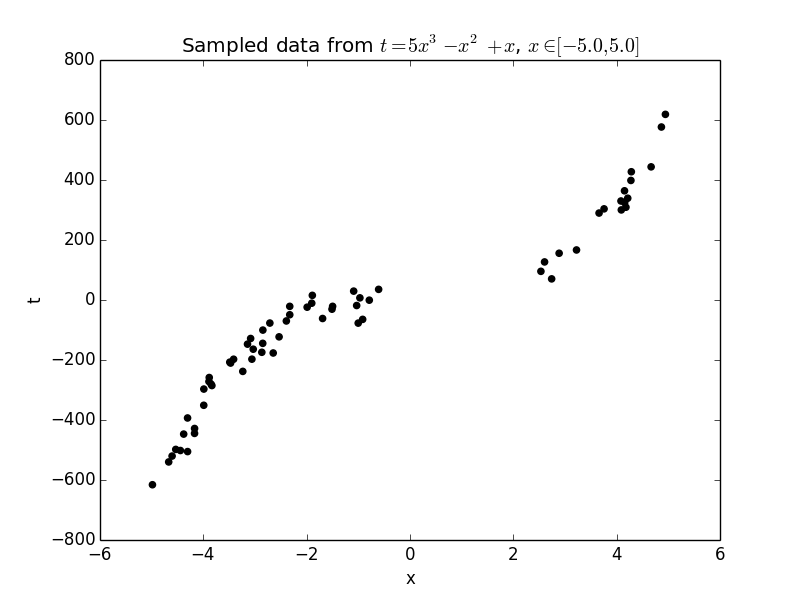
\includegraphics[width=10cm]{figure_6.png}
\caption{This plot is of the data after the data found between $-0.5 \le x \le 2.5$ is removed}
\end{center}
\end{figure}

%% The following can be used for part (b), for displaying multiple figures within a single figure
\begin{figure}[htb]
\begin{center}
\subfigure[]{
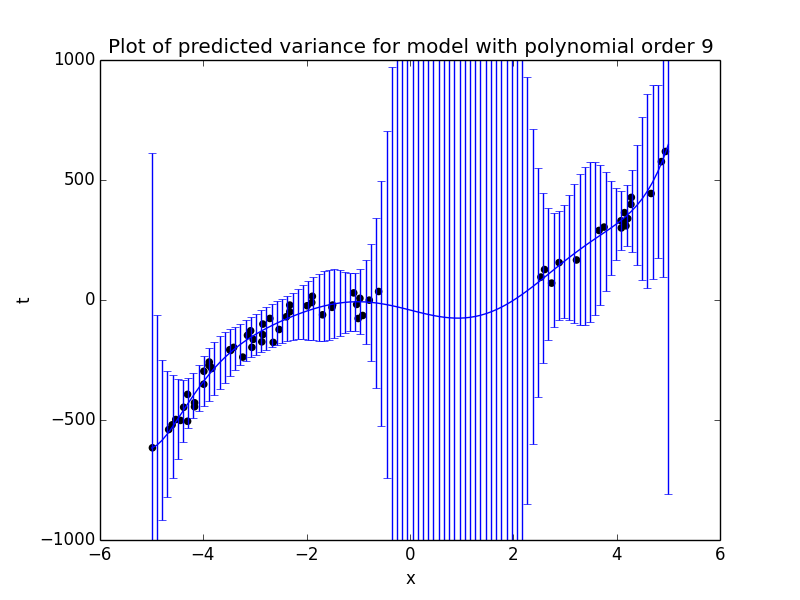
\includegraphics[width=.48\textwidth]{figure_2.png}
}
\subfigure[]{
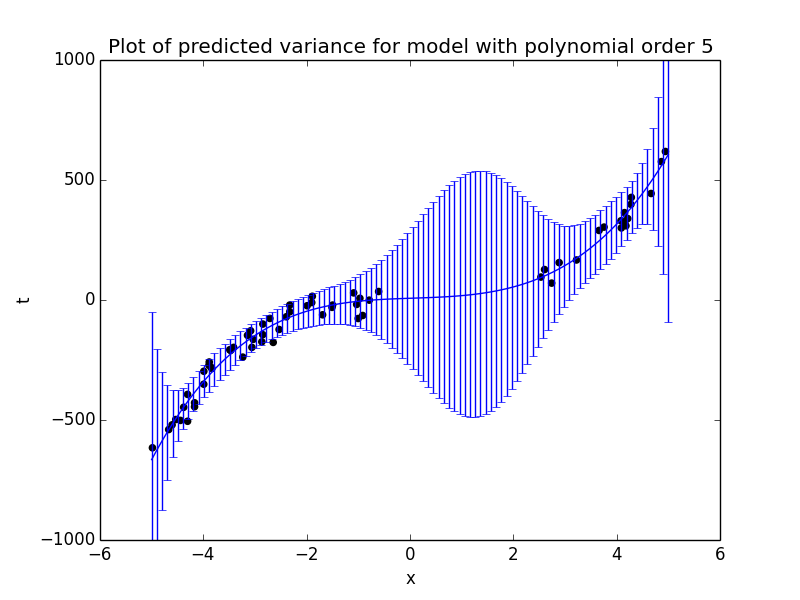
\includegraphics[width=.48\textwidth]{figure_3.png}
}

\subfigure[]{
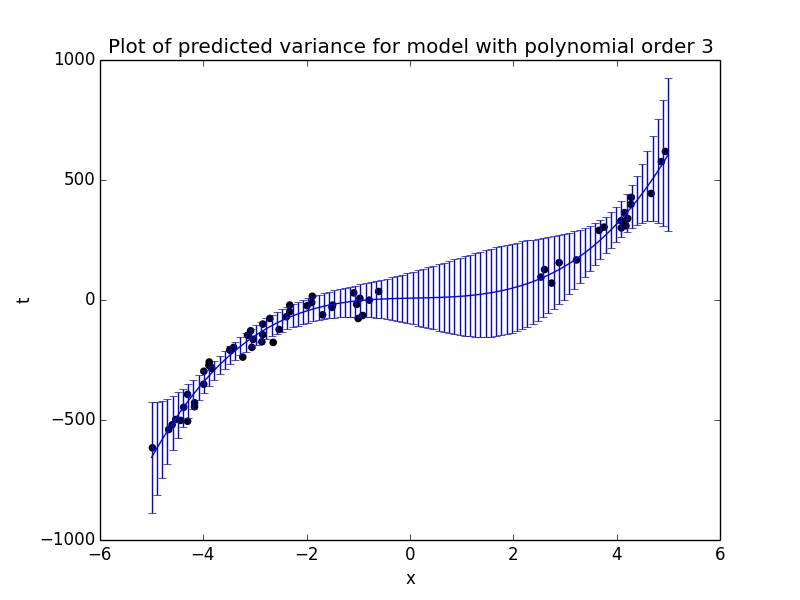
\includegraphics[width=.48\textwidth]{figure_4.png}
}
\subfigure[]{
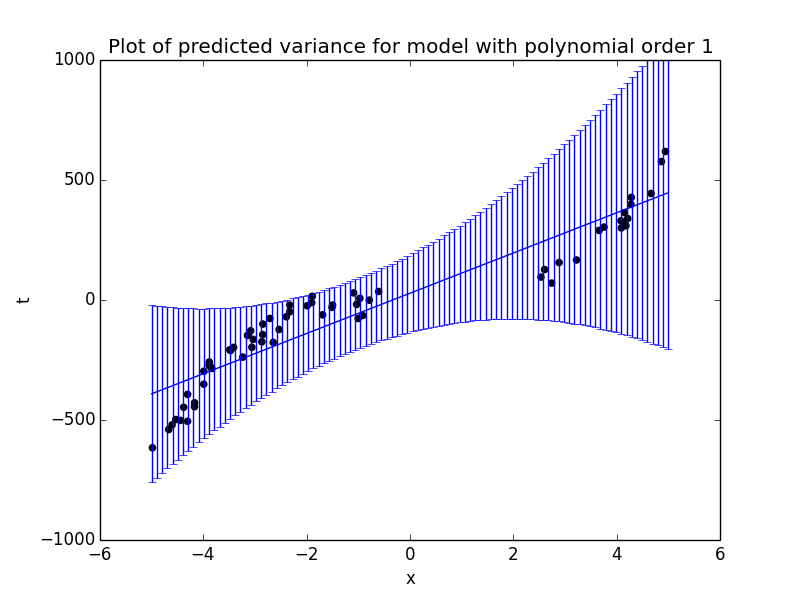
\includegraphics[width=.48\textwidth]{figure_5.png}
}

\caption{Fig a shows the error bars of a $9^{th}$ order regression, note that the error is greatest in the areas at the edge and in the middle, where the data is missing.  Fig b shows similar tendencies but is a $5^{th}$ order regression and more accurate than fig a. Fig c is a $3^{rd}$ order regression and shows the smallest error space, thought the error is still greatest around the missing data.  Fig d is a $1^{st}$ order regression and has the smallest error around the missing data relative to the overall error, but is still less accurate than that of figure c and even fig b. }
\end{center}
\end{figure}

%% The following can be used for part (c), for displaying multiple figures within a single figure
\begin{figure}[htb]
\clearpage
\begin{center}
\subfigure[]{
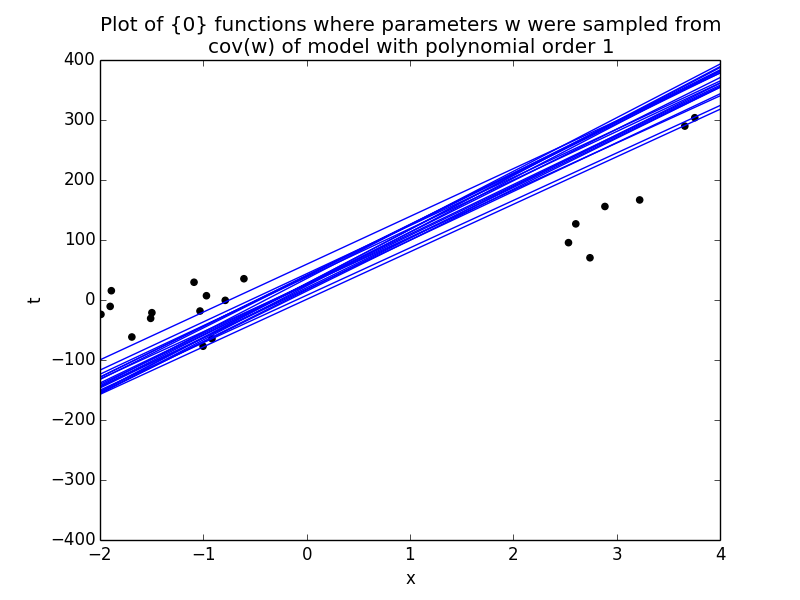
\includegraphics[width=.48\textwidth]{figure_1.png}
}
\subfigure[]{
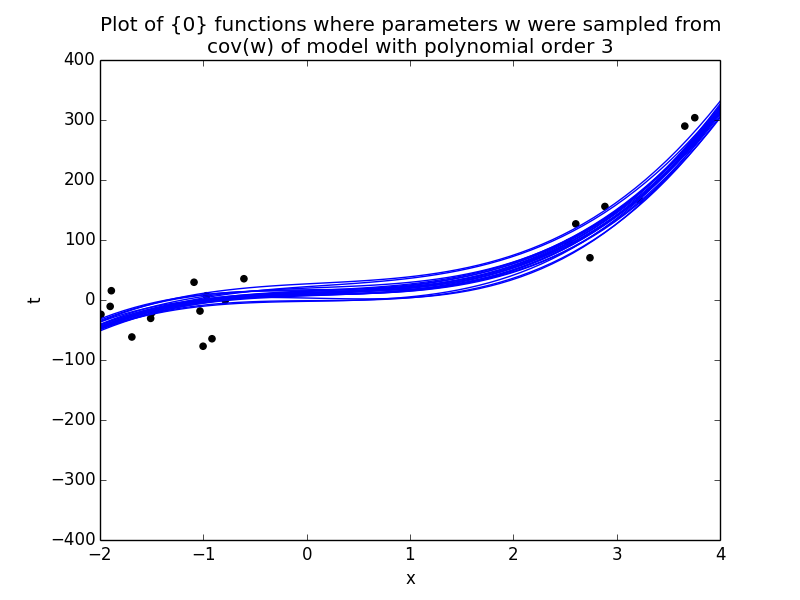
\includegraphics[width=.48\textwidth]{figure_7.png}
}

\subfigure[]{
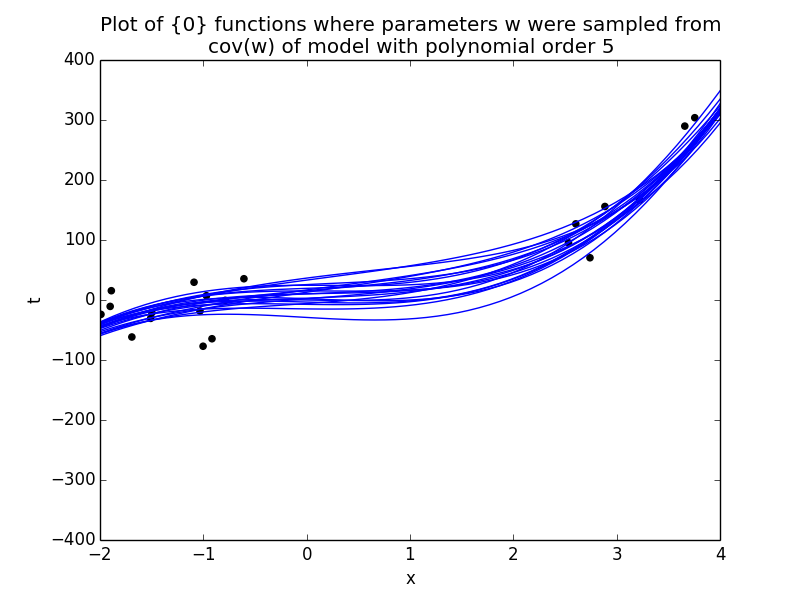
\includegraphics[width=.48\textwidth]{figure_8.png}
}
\subfigure[]{
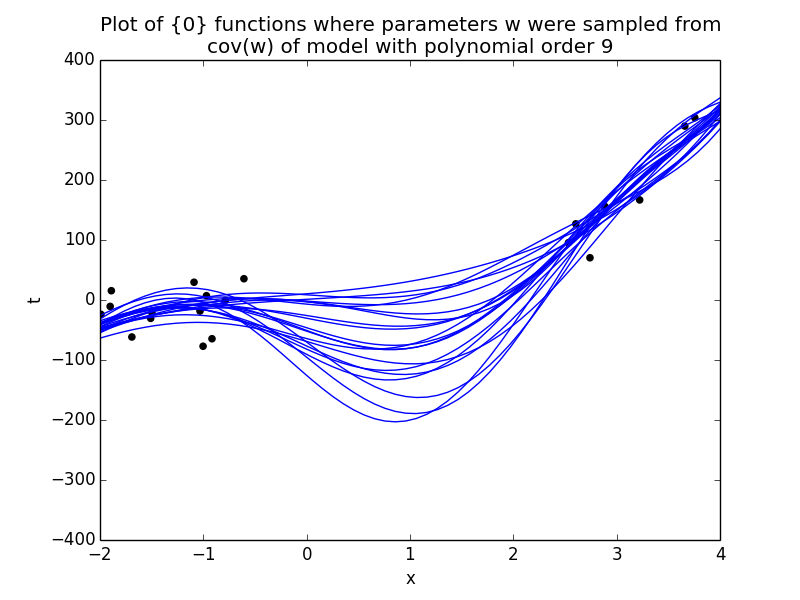
\includegraphics[width=.48\textwidth]{figure_9.png}
}

\caption{Each diagram shows several instances of possible models created by sampling the data, each conform to the error bars seen in the previous diagrams.}
\end{center}
\end{figure}

%%     Problem 7
\clearpage
\item[7.] [5 points]

In this exercise, you will create a simple demonstration of how model bias impacts variance, similar to the demonstration in class.  Using the same true model in the script {\tt predictive\_variance\_example.py}, that is $t = 5x^3-x^2+x$, generate 20 data sets, each consisting of 25 samples from the true function (using the same range of $x \in [-5.0,5.0]$).  Then, create a separate plot for each of the model polynomial orders 1, 3, 5 and 9, in which you plot the true function in red and each of the best fit functions of that model order to the 20 data sets.  You will therefore produce four plots.  The first will be for model order 1 and will include the true model plotted in red and then 20 curves, one each for an order 1 best fit model for each of the 20 data set, for all data sets.  The second plot will repeat this for model order 3, and so on.  You can use any of the code in the script {\tt predictive\_variance\_example.py} as a guide.  Describe what happens to the variance in the functions as the model order is changed.  (tips: plot the true function curve last, so it is plotted on top of the others; also, use {\tt linewidth=3} in the plot fn to increase the line width to make the curve stand out more.)

{\bf Solution.}

%% For latex users: code to insert figure, and update the caption to describe the figure!
%% The following can be used for displaying multiple figures within a single figure
\begin{figure}[htb]
\begin{center}
\subfigure[]{
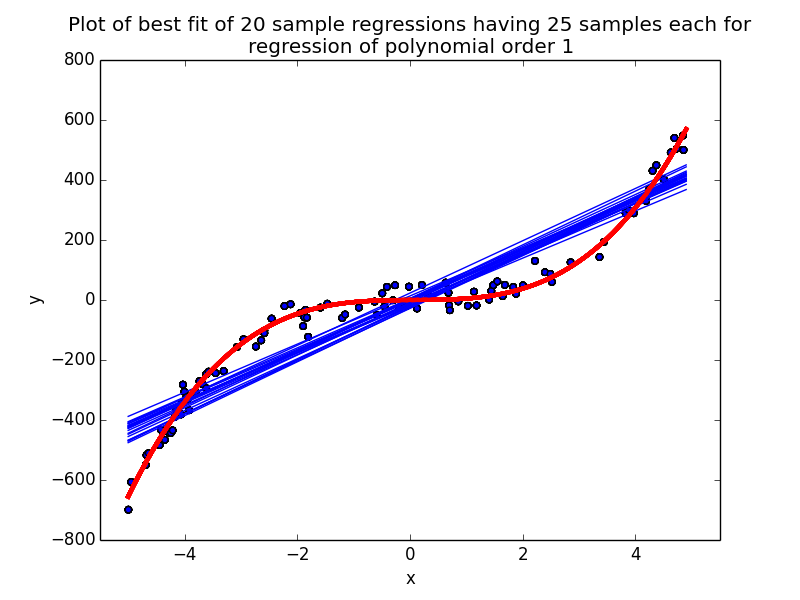
\includegraphics[width=.4\textwidth]{figure_1_7.png}
}
\subfigure[]{
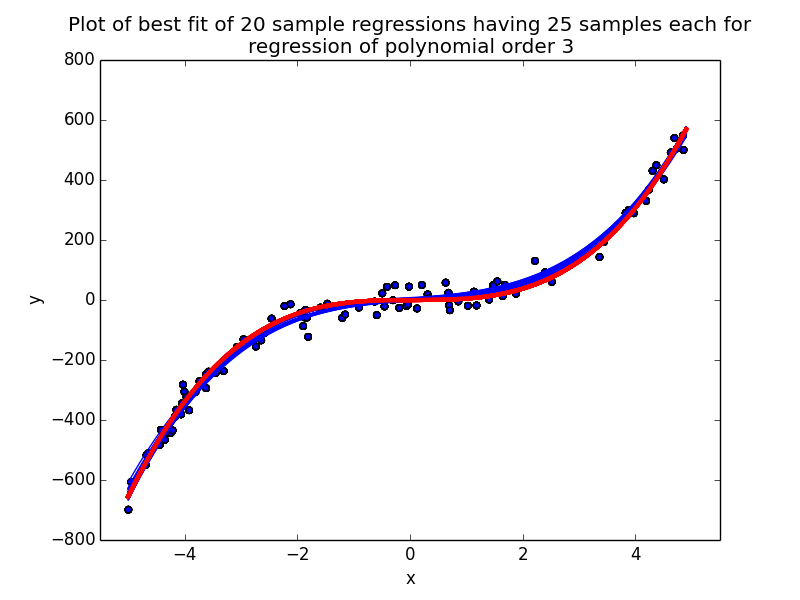
\includegraphics[width=.4\textwidth]{figure_2_7.png}
}

\subfigure[]{
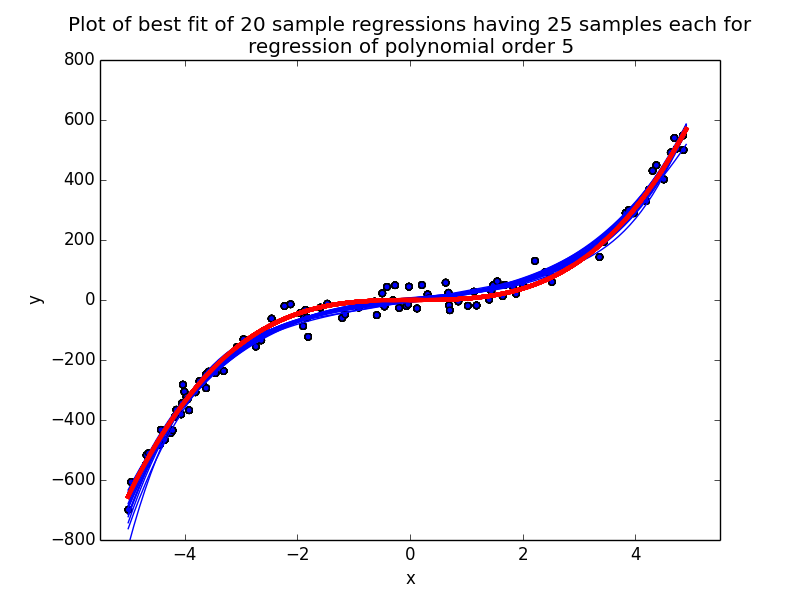
\includegraphics[width=.4\textwidth]{figure_3_7.png}
}
\subfigure[]{
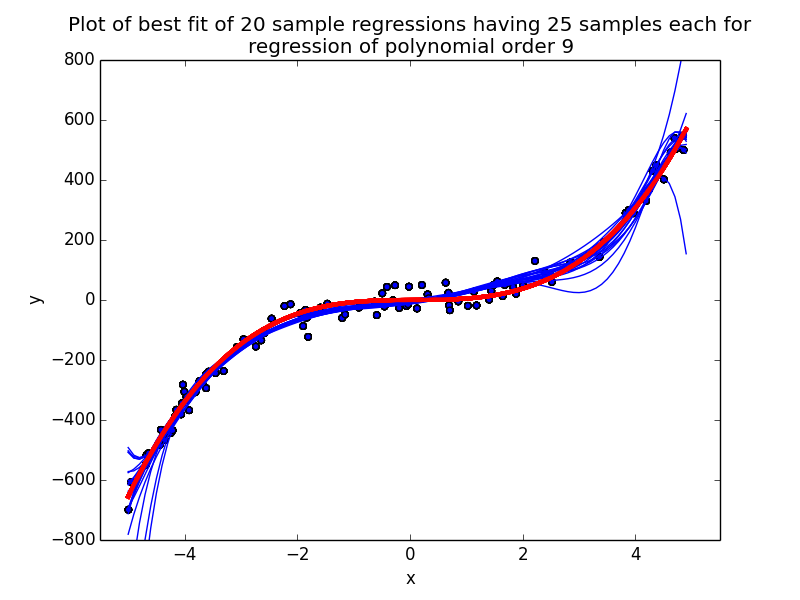
\includegraphics[width=.4\textwidth]{figure_4_7.png}
}

\caption{As seen, the data shows that the regression models conform to a would be predicted variance for each curve with the areas in the center of the distributions more tightly spaced than that of the extremes.  The ideal fit is  the $3^{rd}$ order polynomial wight he least variance, with $5^{th}$ order model coming in a close second.  The $1^{st}$ order regression conforms to the mean values of the sample points, giving it perhaps the poorest fit for prediction, while the $9^{th}$ order polynomial over fits the center of the samples, but diverges wildly at the extremes.  Given the plots provided, I would say that as the order increases to the best model, the models better conform to the data, however as the model's order progresses past the best fit, the potential of for error at the extremes increases with each successive order and moves closer to the center of the sample.}
\end{center}
\end{figure}


%%%     Problem 8
\clearpage
\item[8.] [3 points; \boldred{Required only for Graduates}]
Adapted from {\bf Exercise 2.13} of FCMA p.92:

Compute the Fisher Information Matrix for the parameter of a Bernoulli distribution.

{\bf Solution.} $<$Solution goes here$>$

\end{itemize}

\end{document}